\begin{tikzpicture}[x=1cm,y=1cm]
  % Lienzo global 25.8cm x 17.1cm
  \fill[infPaper] (-0.30,-17.05) rectangle (25.45,0.20);

  % ============================================================================
  % COLUMNA 1: PHILIPPE MEIRIEU (2020) - AZUL MARINO (x = 0.0 .. 8.15)
  % ============================================================================
  \draw[fill=white,draw=infNavy,line width=1.1pt,rounded corners=7pt] (0.0,-15.72) rectangle (8.15,0.0);
  \fill[infNavy,rounded corners=6pt] (0.0,-2.48) rectangle (8.15,0.0);
  \fill[infNavy] (0.0,-2.48) rectangle (8.15,-2.00);
  \node[anchor=north west,text width=5.45cm,align=left,inner sep=0pt] at (0.28,-0.22) {%
    {\color{white}\fontsize{12.5}{14}\selectfont\bfseries Philippe Meirieu\par}\vspace{2pt}%
    {\color{white!90}\fontsize{7.4}{8.8}\selectfont\bfseries «La escuela después»... ¿con la\\pedagogía de antes?\par}\vspace{3pt}%
    {\colorbox{infBlueAccent}{\color{white}\fontsize{6.5}{7.5}\selectfont\bfseries\ 2020 · MCEP de Madrid \ }}%
  };
  \node[inner sep=0pt] at (6.92,-1.24) {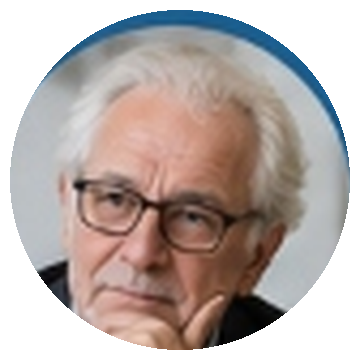
\includegraphics[width=2.06cm]{img_infografia/meirieu_photo.png}};

  % Cintillo subtitulo col 1
  \fill[infBlueLight] (0.12,-3.04) rectangle (8.03,-2.56);
  \node[font=\fontsize{7.0}{8.2}\selectfont\bfseries\color{infNavy}] at (4.075,-2.80) {Repensar la escuela para un mundo en transformación};

  % Idea central col 1
  \InfSectionBar{0.20}{-3.16}{infNavy}{infBlueLight}{target}{Idea central}
  \node[anchor=north west,text width=7.65cm,align=left,font=\fontsize{6.6}{8.0}\selectfont\color{infInk},inner sep=0pt] at (0.25,-3.74) {%
    La crisis puede ser oportunidad para transformar la educación, pero solo si cuestionamos las prácticas que reproducen desigualdad y devolvemos la pedagogía al centro.%
  };

  % Conceptos clave col 1 (4 tarjetas con pictogramas)
  \InfSectionBar{0.20}{-4.86}{infNavy}{infBlueLight}{key}{Conceptos clave}
  \InfConceptCard{0.20}{-5.44}{infNavy}{infBlueCard}{personas}{\textbf{Escuela como bien común}\\Espacio público de encuentro.}
  \InfConceptCard{2.17}{-5.44}{infNavy}{infBlueCard}{autonomia}{\textbf{Autonomía con sentido}\\Se construye con apoyo guiado.}
  \InfConceptCard{4.14}{-5.44}{infNavy}{infBlueCard}{dialogo}{\textbf{Cooperación y alteridad}\\Decir «yo» en un «nosotros».}
  \InfConceptCard{6.11}{-5.44}{infNavy}{infBlueCard}{alerta}{\textbf{Riesgos de retorno}\\Evitar volver a «lo anormal».}

  % Aportes principales col 1
  \InfSectionBar{0.20}{-7.78}{infNavy}{infBlueLight}{bulb}{Aportes principales}
  \InfBullet{0.22}{-8.38}{infNavy}{Formar ciudadanía libre, crítica y solidaria desde conocimientos «infinitamente compartibles» (Fichte).}
  \InfBullet{0.22}{-9.04}{infNavy}{Superar la selección sobre prerrequisitos: motivación y esfuerzo son metas, no filtros de exclusión.}
  \InfBullet{0.22}{-9.70}{infNavy}{Ofrecer «algo más» cara a cara cuando el alumno se bloquea en lugar de repetir «más de lo mismo».}
  \InfBullet{0.22}{-10.36}{infNavy}{La tecnología no sustituye la relación educativa; rechazar el conductismo individualista de pantalla.}

  % Implicaciones para la practica col 1
  \InfSectionBar{0.20}{-11.12}{infNavy}{infBlueLight}{gear}{Implicaciones para la práctica}
  \InfCheck{0.22}{-11.72}{infNavy}{Diseñar debates matemáticos que fomenten ayuda mutua.}
  \InfCheck{0.22}{-12.26}{infNavy}{Atender desigualdades materiales brindando andamiajes accesibles.}
  \InfCheck{0.22}{-12.80}{infNavy}{Evitar rutinas algorítmicas mecánicas sin reflexión conceptual.}
  \InfCheck{0.22}{-13.34}{infNavy}{Sostener una escuela incluyente donde cada estudiante tome la palabra.}

  % Tarjeta inferior col 1
  \fill[infBlueLight,rounded corners=5pt] (0.20,-15.52) rectangle (7.95,-14.05);
  \node[text width=7.35cm,align=center,font=\fontsize{6.6}{8.1}\selectfont\color{infNavy}] at (4.075,-14.78) {%
    \textbf{\textit{«Hacer escuela es hacer sociedad: enseñar la clase para que el mundo sea un mundo de tesoros.»}}\\
    {\scriptsize — Philippe Meirieu (2020)}%
  };

  % ============================================================================
  % COLUMNA 2: KEITH SAWYER (2008) - VERDE ESMERALDA (x = 8.50 .. 16.65)
  % ============================================================================
  \draw[fill=white,draw=infGreen,line width=1.1pt,rounded corners=7pt] (8.50,-15.72) rectangle (16.65,0.0);
  \fill[infGreen,rounded corners=6pt] (8.50,-2.48) rectangle (16.65,0.0);
  \fill[infGreen] (8.50,-2.48) rectangle (16.65,-2.00);
  \node[anchor=north west,text width=5.45cm,align=left,inner sep=0pt] at (8.78,-0.22) {%
    {\color{white}\fontsize{12.5}{14}\selectfont\bfseries Keith Sawyer\par}\vspace{2pt}%
    {\color{white!90}\fontsize{7.4}{8.8}\selectfont\bfseries Aportes de las ciencias del\\aprendizaje\par}\vspace{3pt}%
    {\colorbox{infGreenAccent}{\color{white}\fontsize{6.5}{7.5}\selectfont\bfseries\ 2008 · OECD / CERI \ }}%
  };
  \node[inner sep=0pt] at (15.42,-1.24) {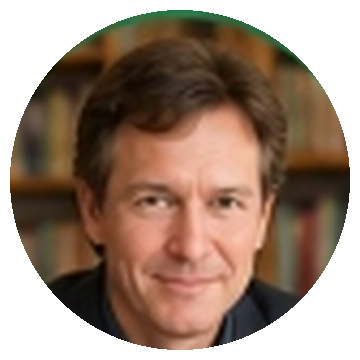
\includegraphics[width=2.06cm]{img_infografia/sawyer_photo.png}};

  \fill[infGreenLight] (8.62,-3.04) rectangle (16.53,-2.56);
  \node[font=\fontsize{7.0}{8.2}\selectfont\bfseries\color{infGreen}] at (12.575,-2.80) {Cómo aprendemos y qué pueden hacer las escuelas};

  \InfSectionBar{8.70}{-3.16}{infGreen}{infGreenLight}{target}{Idea central}
  \node[anchor=north west,text width=7.65cm,align=left,font=\fontsize{6.6}{8.0}\selectfont\color{infInk},inner sep=0pt] at (8.75,-3.74) {%
    El aprendizaje profundo ocurre cuando el estudiantado participa activamente en desafíos auténticos, articula su pensamiento y construye saber en interacción social y andamiada.%
  };

  \InfSectionBar{8.70}{-4.86}{infGreen}{infGreenLight}{key}{Conceptos clave}
  \InfConceptCard{8.70}{-5.44}{infGreen}{infGreenCard}{cerebro}{\textbf{Aprendizaje profundo}\\Comprensión y transferencia real.}
  \InfConceptCard{10.67}{-5.44}{infGreen}{infGreenCard}{construccion}{\textbf{Construcción activa}\\Partir de saberes previos.}
  \InfConceptCard{12.64}{-5.44}{infGreen}{infGreenCard}{dialogo}{\textbf{Interacción social}\\Conocimiento distribuido.}
  \InfConceptCard{14.61}{-5.44}{infGreen}{infGreenCard}{bulb}{\textbf{Creatividad aplicada}\\Analistas simbólicos críticos.}

  \InfSectionBar{8.70}{-7.78}{infGreen}{infGreenLight}{bulb}{Aportes principales}
  \InfBullet{8.72}{-8.38}{infGreen}{Superar el instruccionismo de la era industrial basado en transmisión memorística y pasos mecánicos.}
  \InfBullet{8.72}{-9.04}{infGreen}{Reconocer concepciones previas («matemáticas ingenuas») para reestructurar errores conceptuales.}
  \InfBullet{8.72}{-9.70}{infGreen}{Fomentar articulación oral y escrita, metacognición y andamiaje (\textit{scaffolding}) gradualmente retirado.}
  \InfBullet{8.72}{-10.36}{infGreen}{La evidencia TIMSS demuestra que mayor coherencia conceptual rinde más que currículos saturados.}

  \InfSectionBar{8.70}{-11.12}{infGreen}{infGreenLight}{gear}{Implicaciones para la práctica}
  \InfCheck{8.72}{-11.72}{infGreen}{Plantear retos de modelación ligados a prácticas profesionales.}
  \InfCheck{8.72}{-12.26}{infGreen}{Promover equipos con roles rotativos e interdependencia real.}
  \InfCheck{8.72}{-12.80}{infGreen}{Usar guías decrecientes sin resolver el ejercicio por el alumno.}
  \InfCheck{8.72}{-13.34}{infGreen}{Evaluar comprensión conceptual, coherencia y transferencia.}

  \fill[infGreenLight,rounded corners=5pt] (8.70,-15.52) rectangle (16.45,-14.05);
  \node[text width=7.35cm,align=center,font=\fontsize{6.6}{8.1}\selectfont\color{infGreen}] at (12.575,-14.78) {%
    \textbf{\textit{«Aprendemos mejor cuando externalizamos ideas, colaboramos en comunidad e integramos saberes.»}}\\
    {\scriptsize — R. Keith Sawyer (2008)}%
  };

  % ============================================================================
  % COLUMNA 3: FELIPE MARTÍNEZ RIZO (2026) - TERRACOTA (x = 17.00 .. 25.15)
  % ============================================================================
  \draw[fill=white,draw=infOrange,line width=1.1pt,rounded corners=7pt] (17.00,-15.72) rectangle (25.15,0.0);
  \fill[infOrange,rounded corners=6pt] (17.00,-2.48) rectangle (25.15,0.0);
  \fill[infOrange] (17.00,-2.48) rectangle (25.15,-2.00);
  \node[anchor=north west,text width=5.45cm,align=left,inner sep=0pt] at (17.28,-0.22) {%
    {\color{white}\fontsize{12.0}{14}\selectfont\bfseries Felipe Martínez Rizo\par}\vspace{2pt}%
    {\color{white!90}\fontsize{7.4}{8.8}\selectfont\bfseries Lectura contextualizada de\\PISA 2025\par}\vspace{3pt}%
    {\colorbox{infOrangeAccent}{\color{white}\fontsize{6.5}{7.5}\selectfont\bfseries\ 2026 · Distancia por tiempos \ }}%
  };
  \node[inner sep=0pt] at (23.92,-1.24) {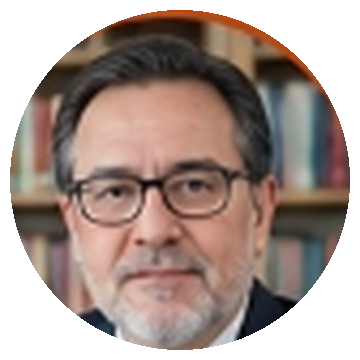
\includegraphics[width=2.06cm]{img_infografia/martinez_photo.png}};

  \fill[infOrangeLight] (17.12,-3.04) rectangle (25.03,-2.56);
  \node[font=\fontsize{7.0}{8.2}\selectfont\bfseries\color{infOrange}] at (21.075,-2.80) {Más allá del puntaje: comprender para mejorar};

  \InfSectionBar{17.20}{-3.16}{infOrange}{infOrangeLight}{target}{Idea central}
  \node[anchor=north west,text width=7.65cm,align=left,font=\fontsize{6.6}{8.0}\selectfont\color{infInk},inner sep=0pt] at (17.25,-3.74) {%
    Los resultados de PISA deben leerse desde su trayectoria histórica, cobertura escolar y contexto social: no son un ranking definitivo, sino insumo para políticas y prácticas justas.%
  };

  \InfSectionBar{17.20}{-4.86}{infOrange}{infOrangeLight}{key}{Conceptos clave}
  \InfConceptCard{17.20}{-5.44}{infOrange}{infOrangeCard}{grafica}{\textbf{Series y contexto}\\PISA 2018--2025 con cautela.}
  \InfConceptCard{19.17}{-5.44}{infOrange}{infOrangeCard}{balanza}{\textbf{Equidad e inclusión}\\Efecto de ampliación escolar.}
  \InfConceptCard{21.14}{-5.44}{infOrange}{infOrangeCard}{doc}{\textbf{Uso evaluativo}\\Orientar mejora, no castigo.}
  \InfConceptCard{23.11}{-5.44}{infOrange}{infOrangeCard}{lupa}{\textbf{Lectura crítica}\\Indagar causas multifactoriales.}

  \InfSectionBar{17.20}{-7.78}{infOrange}{infOrangeLight}{bulb}{Aportes principales}
  \InfBullet{17.22}{-8.38}{infOrange}{Registra descensos en México (lectura $420\to 415\to 408$; matemáticas $409\to 395\to 388$; ciencias $419\to 410\to 414$).}
  \InfBullet{17.22}{-9.04}{infOrange}{Advierte contra rankings alarmistas: comparar sistemas latinoamericanos afines aporta mayor rigor analítico.}
  \InfBullet{17.22}{-9.70}{infOrange}{El aprendizaje responde a factores escolares y extraescolares lentos; la correlación no sustituye explicación causal.}
  \InfBullet{17.22}{-10.36}{infOrange}{Urge reconstruir un sistema nacional propio e independiente que evalúe procesos de aula y escuelas eficaces.}

  \InfSectionBar{17.20}{-11.12}{infOrange}{infOrangeLight}{gear}{Implicaciones para la práctica}
  \InfCheck{17.22}{-11.72}{infOrange}{Usar diagnósticos locales para detectar rezagos comprensivos.}
  \InfCheck{17.22}{-12.26}{infOrange}{Evitar entrenar mecánicamente «para la prueba» estandarizada.}
  \InfCheck{17.22}{-12.80}{infOrange}{Considerar desigualdades de entorno, conectividad y jornada laboral.}
  \InfCheck{17.22}{-13.34}{infOrange}{Articular evaluación formativa cercana con seguimiento continuo.}

  \fill[infOrangeLight,rounded corners=5pt] (17.20,-15.52) rectangle (24.95,-14.05);
  \node[text width=7.35cm,align=center,font=\fontsize{6.6}{8.1}\selectfont\color{infOrange}] at (21.075,-14.78) {%
    \textbf{\textit{«Los datos adquieren sentido cuando se interpretan desde la realidad de las escuelas y las personas.»}}\\
    {\scriptsize — Felipe Martínez Rizo (2026)}%
  };

  % ============================================================================
  % CINTILLO INFERIOR INTEGRADOR + CREDITOS (y = -15.88 .. -16.92)
  % ============================================================================
  \draw[fill=infNavy,draw=infNavy,rounded corners=6pt] (0.0,-16.92) rectangle (25.15,-15.88);
  \node[inner sep=0pt] at (0.72,-16.40) {\InfIconOutline[0.36]{libro}{white}};
  \node[anchor=west,text width=16.8cm,align=left,font=\fontsize{7.4}{8.8}\selectfont\color{white}] at (1.30,-16.40) {%
    \textbf{Tres miradas, un mismo propósito:} una escuela más justa (Meirieu, 2020), con aprendizajes profundos (Sawyer, 2008) y decisiones evaluativas basadas en evidencia contextualizada (Martínez Rizo, 2026).%
  };
  \node[anchor=east,text width=6.4cm,align=right,font=\fontsize{6.1}{7.4}\selectfont\color{white!90}] at (24.90,-16.40) {%
    \textbf{Mtro. Martín Jonathan de la Cruz Muñoz (Matrícula 00874)}\\
    IIIEPE · MAEM · Cohorte SD26 · 19 de noviembre de 2026%
  };
\end{tikzpicture}